% CREATED BY DAVID FRISK, 2015

\chapter{Governing Equations and Solution methods}

\section{Governing Equations}
\subsection{Laplace equation}The Laplace equation in 2D solved in this code is given below,
\begin{equation}\label{eq:uhe}
 \frac{\partial^2 T}{\partial x^2}+\frac{\partial^2 T}{\partial y^2} = 0
\end{equation}

$T$ is any physical variable like Temperature etc., and $x$ and $t$ represent the spatial coordinates.







\section{Numerical Method}
\hspace{0.25cm}The governing equation can be discretised using finite difference method and the final equation is expressed below. 

A standard 5 point stencil is represented by, 
\begin{figure}[H]
\centering
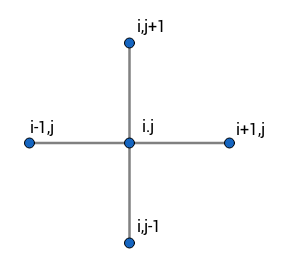
\includegraphics[scale=0.4]{figures/stencil.png}
\caption{five point stencil}
\label{fig:rline}
\end{figure}
Using the above representation, the final equation can be written as,
\begin{equation}
         T_{i,j}+\frac{1}{4}(T_{i,j+1}+T_{i,j-1}+T_{i,j+1}+T_{i,j-1}) 
\end{equation}


    


